\section{Business Relationships with Neighbouring ISPs}
\label{sec:relationships}

BT Network has three immediate neighbouring ISPs and it's important to form business relationships with all three of them in order to gain economic benefits. 
The external routing policies of BGP protocol for each outside network are determined by the business relationship with which our network is connected to (see Section \ref{sec:bgp} for details).
Our business relationships with neighbouring ISPs are shown in Figure \ref{fig:relationships} and elaborated in the following.

\begin{figure*}[ht!]
    \centering
    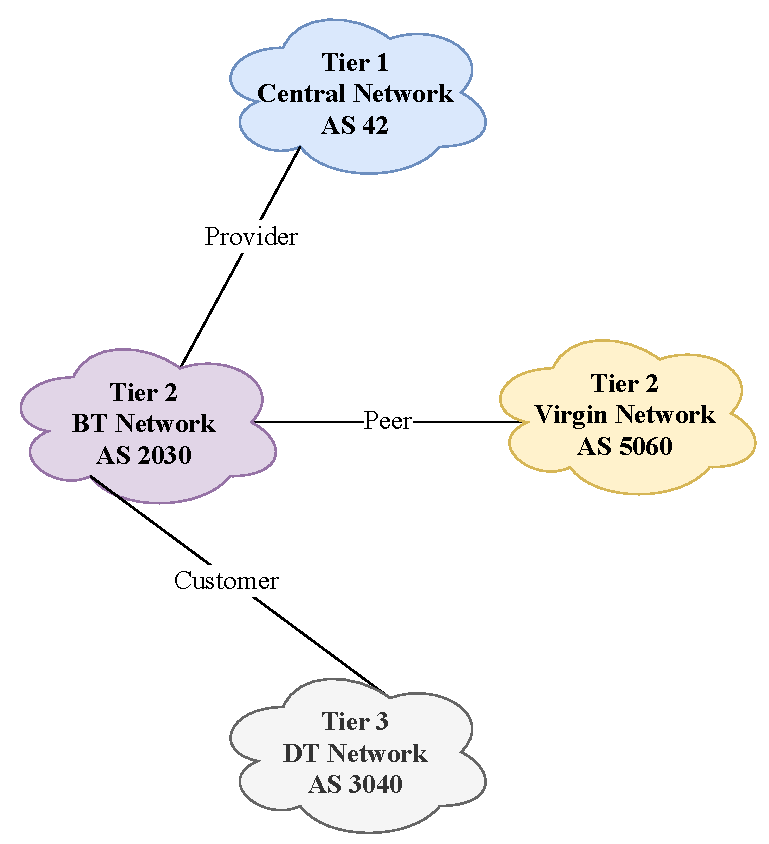
\includegraphics[width=0.5\linewidth]{relationships}
    \caption{Business Relationships of BT Network with Neighbouring ISPs.}
    \label{fig:relationships}
\end{figure*}


\subsection{Provider: Central Network}
Since BT Network is a Tier-2 ISP, it need to be connected to a Tier-1 ISP to gain wider Internet connection. Therefore, BT is connected to Central Network as a customer, a Tier-1 ISP, which makes Central Network a network provider for BT.

\subsection{Peer: Virgin Network}
BT Network forms a Peer relationship with Virgin Network, which allows Virgin Network to connect to BT Network at zero cost and vice versa.

\subsection{Customer: DT Network}
\label{sec:dt}
BT Network forms a Provider-Customer relationship with DT Network, in which BT is the provider and DT is the customer. In other words, DT gains access to the border Internet through BT at a cost.
